% GNUPLOT: LaTeX picture with Postscript
\begingroup
  \makeatletter
  \providecommand\color[2][]{%
    \GenericError{(gnuplot) \space\space\space\@spaces}{%
      Package color not loaded in conjunction with
      terminal option `colourtext'%
    }{See the gnuplot documentation for explanation.%
    }{Either use 'blacktext' in gnuplot or load the package
      color.sty in LaTeX.}%
    \renewcommand\color[2][]{}%
  }%
  \providecommand\includegraphics[2][]{%
    \GenericError{(gnuplot) \space\space\space\@spaces}{%
      Package graphicx or graphics not loaded%
    }{See the gnuplot documentation for explanation.%
    }{The gnuplot epslatex terminal needs graphicx.sty or graphics.sty.}%
    \renewcommand\includegraphics[2][]{}%
  }%
  \providecommand\rotatebox[2]{#2}%
  \@ifundefined{ifGPcolor}{%
    \newif\ifGPcolor
    \GPcolortrue
  }{}%
  \@ifundefined{ifGPblacktext}{%
    \newif\ifGPblacktext
    \GPblacktextfalse
  }{}%
  % define a \g@addto@macro without @ in the name:
  \let\gplgaddtomacro\g@addto@macro
  % define empty templates for all commands taking text:
  \gdef\gplbacktext{}%
  \gdef\gplfronttext{}%
  \makeatother
  \ifGPblacktext
    % no textcolor at all
    \def\colorrgb#1{}%
    \def\colorgray#1{}%
  \else
    % gray or color?
    \ifGPcolor
      \def\colorrgb#1{\color[rgb]{#1}}%
      \def\colorgray#1{\color[gray]{#1}}%
      \expandafter\def\csname LTw\endcsname{\color{white}}%
      \expandafter\def\csname LTb\endcsname{\color{black}}%
      \expandafter\def\csname LTa\endcsname{\color{black}}%
      \expandafter\def\csname LT0\endcsname{\color[rgb]{1,0,0}}%
      \expandafter\def\csname LT1\endcsname{\color[rgb]{0,1,0}}%
      \expandafter\def\csname LT2\endcsname{\color[rgb]{0,0,1}}%
      \expandafter\def\csname LT3\endcsname{\color[rgb]{1,0,1}}%
      \expandafter\def\csname LT4\endcsname{\color[rgb]{0,1,1}}%
      \expandafter\def\csname LT5\endcsname{\color[rgb]{1,1,0}}%
      \expandafter\def\csname LT6\endcsname{\color[rgb]{0,0,0}}%
      \expandafter\def\csname LT7\endcsname{\color[rgb]{1,0.3,0}}%
      \expandafter\def\csname LT8\endcsname{\color[rgb]{0.5,0.5,0.5}}%
    \else
      % gray
      \def\colorrgb#1{\color{black}}%
      \def\colorgray#1{\color[gray]{#1}}%
      \expandafter\def\csname LTw\endcsname{\color{white}}%
      \expandafter\def\csname LTb\endcsname{\color{black}}%
      \expandafter\def\csname LTa\endcsname{\color{black}}%
      \expandafter\def\csname LT0\endcsname{\color{black}}%
      \expandafter\def\csname LT1\endcsname{\color{black}}%
      \expandafter\def\csname LT2\endcsname{\color{black}}%
      \expandafter\def\csname LT3\endcsname{\color{black}}%
      \expandafter\def\csname LT4\endcsname{\color{black}}%
      \expandafter\def\csname LT5\endcsname{\color{black}}%
      \expandafter\def\csname LT6\endcsname{\color{black}}%
      \expandafter\def\csname LT7\endcsname{\color{black}}%
      \expandafter\def\csname LT8\endcsname{\color{black}}%
    \fi
  \fi
  \setlength{\unitlength}{0.0500bp}%
  \begin{picture}(5040.00,3770.00)%
    \gplgaddtomacro\gplbacktext{%
    }%
    \gplgaddtomacro\gplfronttext{%
      \csname LTb\endcsname%
      \put(4601,2769){\makebox(0,0)[r]{\strut{}$\frac{\partial^2 f}{\partial xy}$ (numeric)}}%
      \csname LTb\endcsname%
      \put(4601,2549){\makebox(0,0)[r]{\strut{}       8}}%
      \csname LTb\endcsname%
      \put(4601,2329){\makebox(0,0)[r]{\strut{}       6}}%
      \csname LTb\endcsname%
      \put(4601,2109){\makebox(0,0)[r]{\strut{}       4}}%
      \csname LTb\endcsname%
      \put(4601,1889){\makebox(0,0)[r]{\strut{}       2}}%
      \csname LTb\endcsname%
      \put(4601,1669){\makebox(0,0)[r]{\strut{}       0}}%
      \csname LTb\endcsname%
      \put(4601,1449){\makebox(0,0)[r]{\strut{}      -2}}%
      \csname LTb\endcsname%
      \put(4601,1229){\makebox(0,0)[r]{\strut{}      -4}}%
      \csname LTb\endcsname%
      \put(4601,1009){\makebox(0,0)[r]{\strut{}      -6}}%
      \csname LTb\endcsname%
      \put(4601,789){\makebox(0,0)[r]{\strut{}      -8}}%
      \csname LTb\endcsname%
      \put(773,974){\makebox(0,0){\strut{}$0$}}%
      \put(1264,923){\makebox(0,0){\strut{}$0.2$}}%
      \put(1756,871){\makebox(0,0){\strut{}$0.4$}}%
      \put(2247,819){\makebox(0,0){\strut{}$0.6$}}%
      \put(2738,768){\makebox(0,0){\strut{}$0.8$}}%
      \put(3230,716){\makebox(0,0){\strut{}$1$}}%
      \put(1850,762){\makebox(0,0){\strut{}$x$}}%
      \put(3431,788){\makebox(0,0)[l]{\strut{}$0$}}%
      \put(3610,930){\makebox(0,0)[l]{\strut{}$0.2$}}%
      \put(3788,1072){\makebox(0,0)[l]{\strut{}$0.4$}}%
      \put(3967,1214){\makebox(0,0)[l]{\strut{}$0.6$}}%
      \put(4146,1355){\makebox(0,0)[l]{\strut{}$0.8$}}%
      \put(4325,1497){\makebox(0,0)[l]{\strut{}$1$}}%
      \put(4363,1101){\makebox(0,0){\strut{}$y$}}%
      \put(718,1536){\makebox(0,0)[r]{\strut{}$-10$}}%
      \put(718,1630){\makebox(0,0)[r]{\strut{}$-8$}}%
      \put(718,1723){\makebox(0,0)[r]{\strut{}$-6$}}%
      \put(718,1817){\makebox(0,0)[r]{\strut{}$-4$}}%
      \put(718,1910){\makebox(0,0)[r]{\strut{}$-2$}}%
      \put(718,2003){\makebox(0,0)[r]{\strut{}$0$}}%
      \put(718,2096){\makebox(0,0)[r]{\strut{}$2$}}%
      \put(718,2190){\makebox(0,0)[r]{\strut{}$4$}}%
      \put(718,2283){\makebox(0,0)[r]{\strut{}$6$}}%
      \put(718,2377){\makebox(0,0)[r]{\strut{}$8$}}%
      \put(718,2470){\makebox(0,0)[r]{\strut{}$10$}}%
    }%
    \gplbacktext
    \put(0,0){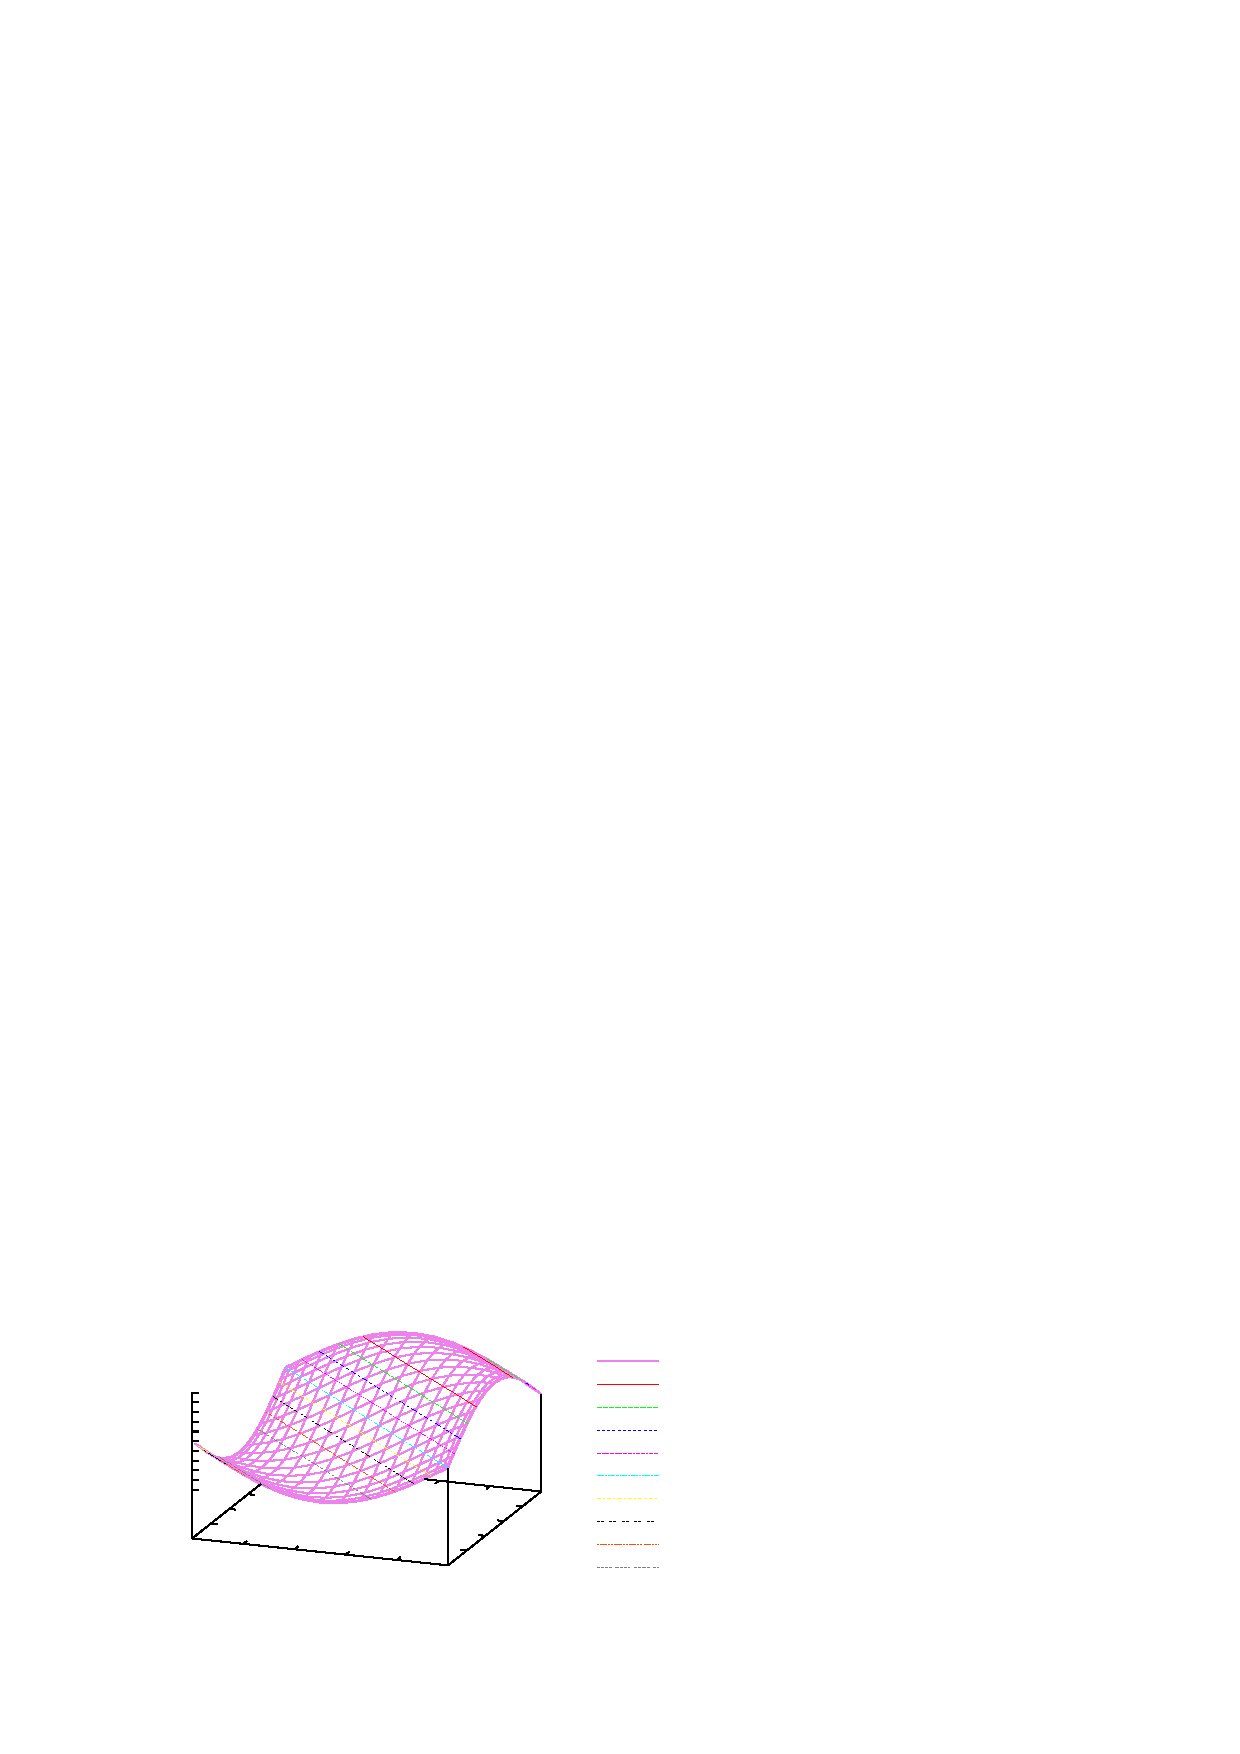
\includegraphics{d2dxy_trnfm_nu}}%
    \gplfronttext
  \end{picture}%
\endgroup
